%%%%%%
%
% $Autor: Wings $
% $Datum: 2021-05-14 $
% $Pfad: GitLab/MLEdgeComputer/Portenta $
% $Dateiname: VisionShield
% $Version: 4620 $
%
%%%%%%



\section{Arduino Portenta Vision Shield}


The vision shield is a hardware add-on to the portenta h7 board in order to perform machine vision applications. It has a camera module with 324X324 pixel resolution which contain ultra-low power image sensor and is highly sensitive in detecting motion, gestures, and object identification. It also has a JTAG connector  to perform debugging or getting special firmware for the board.   In addition, it also has  two on-board microphones for sound detection and analysis in real-time. It is available in two variants : one with Ethernet port for WiFi connectivity and the other with LoRa connectivity. 

In order to perform machine vision applications, Arduino has partnered with OpenMV to provide free license for the OpenMV IDE. OpenMV enables us to develop low-cost MicroPython based machine vision applications. It also has MicroSD slot in order to save programs on it.\cite{VisionShield:2021}


\textbf{Technical Specifications}
\begin{itemize}
	\item Camera: Himax HM-01B0 camera module
	\item Resolution: 320 x 320 active pixel resolution with support for QVGA
	\item Image sensor: Highly sensitive 3.6 µ BrightSenseTM pixel technology
	\item Microphones: 2x MP34DT06JTR
	\item Connection: LAN
	\item Interface: JTAG
	\item Dimensions (LxW): 66 x 25 mm 
\end{itemize}
	\subsection{Camera Module} 
	It has a very low power monochrome  camera with a  maximum of 60 fps and also allows the possibility to perform motion detection without interacting with the main processor. With its “Always on” functionality it switches on the main processor only  when it detects motion and therefore enabling minimum power consumption. It captures images of size 324X324 pixels but this image is cropped down to OpenMV standard resolutions 320X240 which is QVGA(Quarter Video graphics Array). As the name suggests, QVGA is the quarter of the standard VGA which is 640X480 pixels.
	\subsection{Microphones} 
	The microphones present in the vision shield are omnidirectional which means they can receive audio signals in all directions. These features can be used in applications such as speech recognition and predictive maintenance of machines based on the abnormal sounds made by them in an industry.
	\subsection{Micro SD card} 
	The vision shield comes with a micro SD card slot to store images and videos captured by it or read configuration files. 
	
	\subsection{Ethernet}
	The vision shield module with Ethernet connector allows connecting to 10/100 Tx base networks with the help of Ethernet PHY available on the Arduino Portenta H7 board. This enables it connect to the internet using RJ45 cable.
	
	\subsection{LoRa Module}
	The vision shield also comes with a LoRa(Long Range) module variant provided by the Murata CMWX1ZZABZ module which contains STM32L0 processor along with a Semtech SX1276 Radio. With the help of this module we can run computer vision applications wirelessly via LoRa to the cloud.
	\subsection{Power}
	The Arduino Portenta H7 supplies 3.3 Volts power via the output pin(3.3V) to the microSD card slot,dual microphones and LoRa module(ASX00026 only) via the high density conector. An onboard Low-Dropout(LDO) regulator supplies 2.8V output to the camera module.
	
	


\begin{figure}
	\centering
  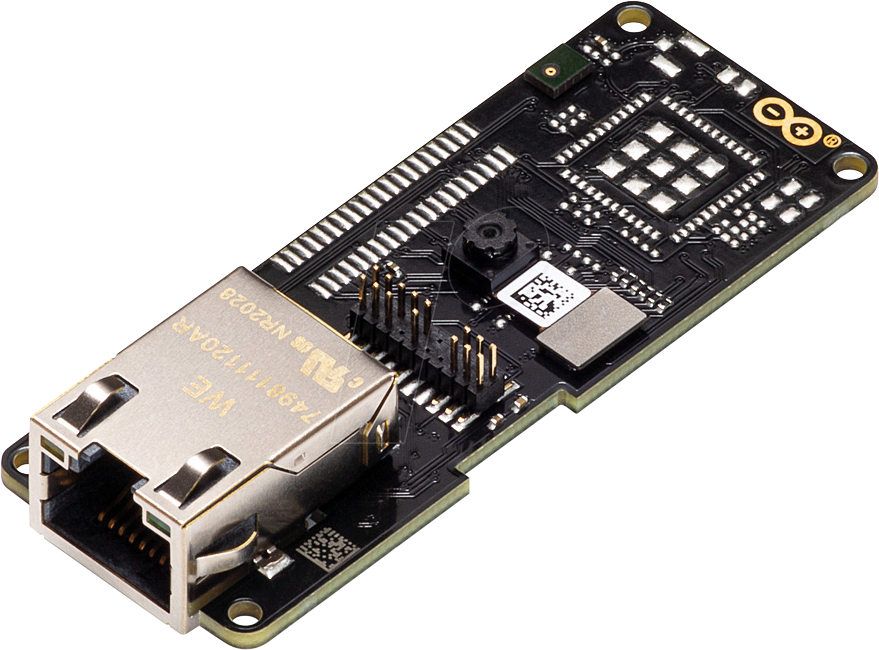
\includegraphics[width=0.4\textwidth]{Arduino/PortentaVisionShield}
\caption{Arduinos Vision Shield für den Portenta H7 \href{https://store.arduino.cc/portenta-h7}{Arduino Store}}
\end{figure}

\begin{figure}
	\centering
	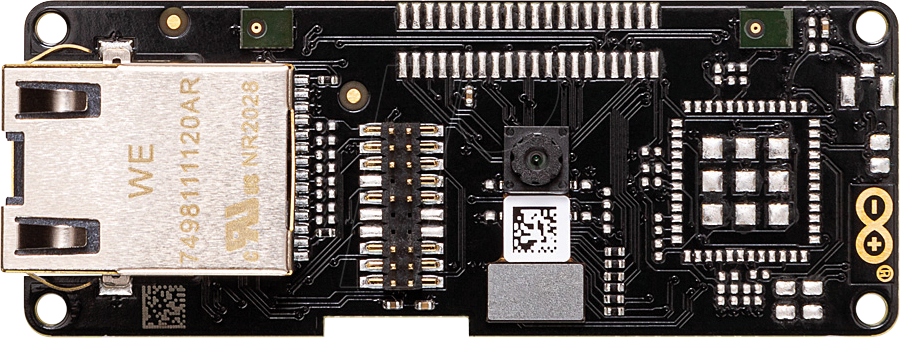
\includegraphics[width=0.4\textwidth]{Arduino/PortentaVisionShield2}
	\caption{Arduinos Vision Shield für den Portenta H7 \href{https://store.arduino.cc/portenta-h7}{Arduino Store}}
\end{figure}

\url{https://www.reichelt.de/arduino-portenta-shield-vision-mit-lan-ard-shd-asx00021-p292402.html?CCOUNTRY=445&LANGUAGE=de&trstct=pos_3&nbc=1&&r=1}


ARD SHD ASX00021

Portenta Vision Shield: eine produktionsreife Lösung für Embedded ML-Anwendungen in Kombination mit dem Arduino Portenta H7 Board

Das Vision Shield wird mit einem 324 x 324 Pixel großen Kameramodul geliefert, das einen Ultra Low Power-Bildsensor enthält, der für Always-on-Vision-Geräte und -Anwendungen entwickelt wurde. Die hochempfindlichen Bildsensoren können Gesten, Umgebungslicht, Näherungserkennung und Objektidentifikation erfassen.

• professionelle Bildverarbeitung
• gerichtete Audioerkennung
• Ethernet oder LoRa (je nach Shield)
• JTAG
• für Arduino Portenta

Arduino hat sich mit OpenMV zusammengetan, um eine kostenlose Lizenz für die OpenMV-IDE anzubieten, die mit MicroPython einen einfachen Einstieg in die Bildverarbeitung ermöglicht. Mit OpenMV können alle Fachleute, Forscher und Entwickler kostengünstige Python-basierte Kamera-Vision- und Audio-Anwendungen entwickeln. Mit den beiden in alle Richtungen integrierten Digitalmikrofonen können Sie Töne zu den Videos aufnehmen, welche auf einer MicroSD-Karte gespeichert werden können.

Übertragen Sie Daten entweder über Ethernet- oder LoRa®
ARD SHD ASX00021 (Shield mit LAN)
ARD SHD ASX00026 (Shield mit LoRa)

Technische Daten
• Kamera: Himax HM-01B0 Kameramodul
• Auflösung: 320 x 320 aktive Pixelauflösung mit Unterstützung für QVGA
• Bildsensor: Hochempfindliche 3,6-µ-BrightSenseTM-Pixeltechnologie
• Mikrofone: 2x MP34DT06JTR
• Verbindung: LAN
• Schnittstelle: JTAG
• Maße (LxB): 66 x 25 mm

Lieferumfang
Portenta Shield mit LAN-Funktion
